\section{Systemfunktionen}
Wir haben die Systemfunktionen nach Usergruppen aufgeteilt. TODO: Hier kommt das Use-Case Diagramm hin!


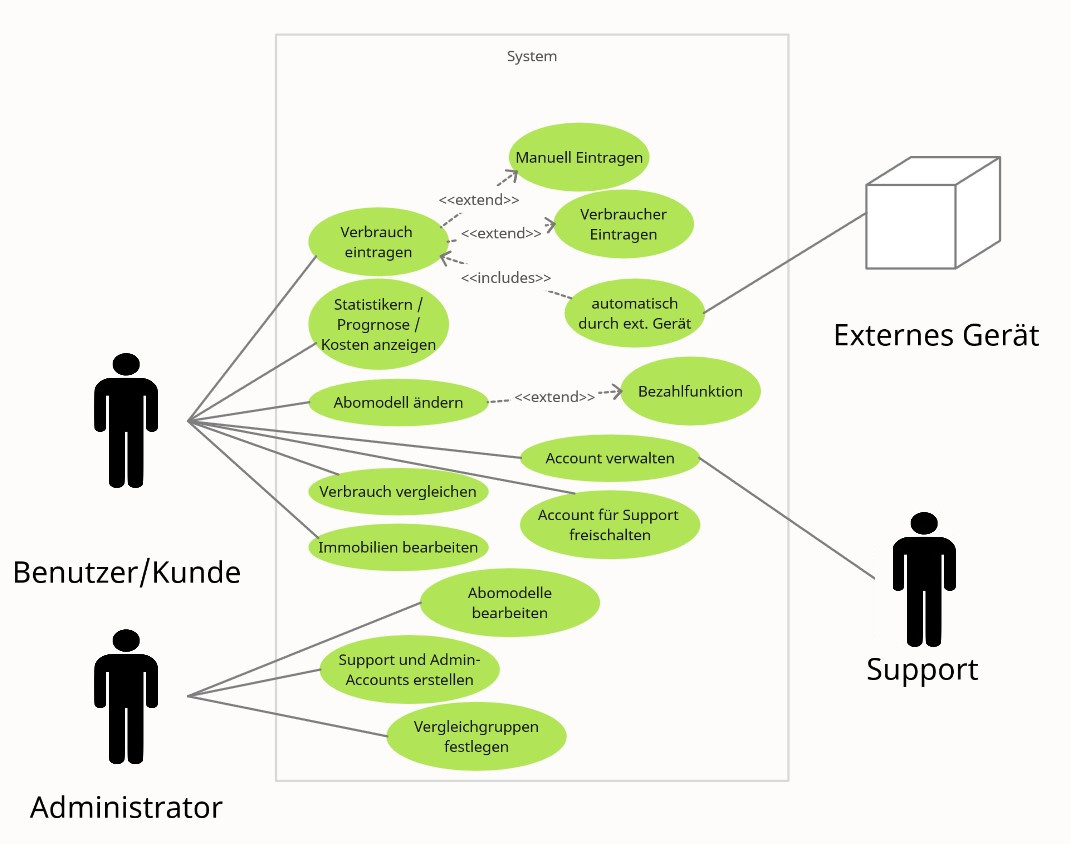
\includegraphics[width=10cm]{system_features/UC.jpg}

\subsection{Systemfunktionen für alle Usergruppen}
\subsubsection{Anmeldung}
\paragraph{Beschreibung und Priorität}
\paragraph{Sequenzen von Benutzeraktionen und Systemantworten}
\paragraph{Funktionale Anforderungen}

\subsection{Benutzer}
\subsubsection{Accounterstellung}
\paragraph{Beschreibung und Priorität}
Diese Funktion ermöglicht es, einer Person, die an dem Produkt interessiert ist, ein Account anzulegen und somit anfangen kann das Produkt zu nutzen. Die Priorität dieser Funktion kann nicht überschätzt werden, da ohne sie, keine der Folgenden umsetzbar wäre.
\paragraph{Sequenzen von Benutzeraktionen und Systemantworten} Der/die Interessierte gibt in der Anmelde-Maske ihren frei gewählten Benutzername, ihre E-Mail-Adresse und schließlich ein Passwort ein. Nach einem Knopfdruck, wird, wenn die Eingaben die funktionalen Anforderungen REG4, REG5, REG6 erfüllen, der Benutzer nun auf die Startseite weitergeleitet. Wenn nicht, wird der Benutzer über die nicht erfüllten Anforderungen in der Anmelde-Maske informiert und kann daraufhin seine/ihre Eingaben anpassen.
\paragraph{Funktionale Anforderungen}
\begin{itemize}
	\item \textbf{REG1} Darstellen der Anmelde-Maske
	\item \textbf{REG2} Validieren den Eingabe also Überprüfung von REG4, REG5, REG6  durch ggf. Abgleich mit der Datenbank
	\item \textbf{REG3} Auf nicht erfüllte Anforderungen (REG4, REG5, REG6) in der Anmeldemaske aufmerksam machen, falls diese nicht erfüllt sind.
	\item \textbf{REG4} Kein 2 Benutzer dürfen den selben Benutzername haben.
	\item \textbf{REG5} Das Passwort muss dem folgenden Standard genügen:
	      \begin{itemize}
		      \item Mindestlänge: 8 Zeichen
		      \item Enthält min. einen deutschen Großbuchstaben (A-Z, Ä, Ö, Ü)
		      \item Enthält min. einen deutschen Kleinbuchstaben (a-z, ä, ö, ü, ß)
		      \item Enthält min. eine arabische Ziffer (0-9)
		      \item Enthält min. ein Zeichen, dass nicht in die bisherigen Kategorien passt (!, \$, \#, \%, ...)
	      \end{itemize}
	\item \textbf{REG6} Die eingegebene E-Mail-Adresse muss im richtigen Format sein.

\end{itemize}

\subsubsection{Verbräuche eintragen}
\paragraph{Beschreibung und Priorität}
Es ermöglicht dem Benutzer seine Daten in die Datenbank einzutragen, welche später für weitere Features von nöten sind. Neben dem manuellen Eintragen gibt es auch die Möglichkeit der automatischen Erfassung der Daten mittels einem Gerät, das der Benutzer zuhause installieren muss, sobald dies passiert ist übermittelt das Gerät jeden Tag die aktuellen Daten… oder so.

\paragraph{Sequenzen von Benutzeraktionen und Systemantworten}
Der Benutzer trägt in einer WebMaske seine einzelnen Verbräuche ein und kann mit einem Klick auf den Button “hochladen” seine Daten der Datenbank hinzufügen, bevor dies geschieht, wird aber überprüft, ob die Daten neu und sinnig sind.
\paragraph{Funktionale Anforderungen}

\subsubsection{Statistiken einsehen}
\paragraph{Beschreibung und Priorität}
\paragraph{Sequenzen von Benutzeraktionen und Systemantworten}
\paragraph{Funktionale Anforderungen}

\subsubsection{Immobilien bearbeiten}
\paragraph{Beschreibung und Priorität}
\paragraph{Sequenzen von Benutzeraktionen und Systemantworten}
\paragraph{Funktionale Anforderungen}

\subsubsection{Abomodell ändern}

\begin{tikzpicture}[object/.style = {draw, rectangle}, activity/.style = {draw, rounded corners=0.1cm}, split/.style = {draw, diamond}, node distance=1.3cm]
	\node[circle, fill] (start) {};
	\node[object] (1) [below of=start] {Abomodell ändern};
	\node[activity] (2) [right of=1, node distance=4cm] {Modell wählen};
	\node[activity] (3) [right of=2, node distance=4cm] {Startzeitpunkt wählen};
	\node[split] (s1) [below of=1] {};
	\node[split] (s2) [below of=s1] {};
	\node[activity] (4) [right of=s2, node distance=5cm] {Modell auf \textit{Frei} setzen};
	\node[circle, fill] (unabo) [right of=4, , node distance=3cm] {};
	\node[split] (s3) [below of=s2] {};
	\node[activity] (5) [right of=s3, node distance=6cm] {Rechnungsadresse eintragen};
	\node[split] (s4) [below of=s3] {};
	\node[activity] (6) [below of=s4] {Bezahlungmethode wählen};
	\node[activity] (7) [right of=6,  node distance=5cm] {Bezahlung durchführen};
	\node[split] (s5) [right of=7,  node distance=3.5cm] {};
	\node[object] (8) [below of=s5, node distance=1.5cm] {Bestätigung};
	\node[activity] (9) [right of=s4, node distance=7.3cm] {Abbrechen};
	\node[circle, fill] [right of=9, node distance=1.35cm] (cancel) {};
	\node[activity] (10) [left of=8, node distance=3cm] {Abomodell setzen};
	\node[circle, fill] [left of=10, node distance=2cm] (finish) {};


	\draw[->] (start) -- (1);
	\draw[->] (1) -- (2);
	\draw[->] (2) -- (3);
	\draw[->] (3) -- (s1);
	\draw[->] (s1) to [out=0,in=270, looseness=0.3] node[below=1mm, align=center] {Startzeitpunkt genügt ABO3 nicht} (3) ;
	\draw[->] (s1) -- node[left=1mm, align=center] {Startzeitpunkt\\genügt ABO3} (s2);
	\draw[->] (s2) -- node[above=1mm] {\textit{Frei} gewählt} (4);
	\draw[->] (4) -- (unabo);
	\draw[->] (s2) -- node[left=1mm, align=center] {gew. Abo \\ kostenpflichtig} (s3);
	\draw[->] (s3) -- node[above=1mm] {Adresse unbekannt} (5);
	\draw[->] (s3) -- node[left=1mm, align=center] {Adresse \\ bekannt} (s4);
	\draw[->] (5) -- (s4);
	\draw[->] (s4) -- node[left=1mm] {kein Abbruch} (6);
	\draw[->] (6) -- (7);
	\draw[->] (7) -- (s5);
	\draw[->] (s5) -- node[left=1mm, align=center] {Zahlung erfolgt} (8);
	\draw[->] (s5) to [out=90,in=0,looseness=0.1] node[right=4.5cm, above=-0.5cm, align=center] {Zahlung abgelehnt} (s4);
	\draw[->] (s4)-- node[above=0.1mm] {\qquad Abbruch} (9);
	\draw[->] (9) --(cancel);
	\draw[->] (8) --(10);
	\draw[->] (10) -- (finish);
\end{tikzpicture}
\paragraph{Beschreibung und Priorität}
Der Benutzer kann hiermit zwischen Abomodellen wechseln. Geplant sind die Abomodelle \textit{Frei}, \textit{Standart} und \textit{Professionell} wovon Ersteres kostenlos und standardmäßig ausgewählt sein sollte. Diese Finktion enthält neben dem Auswählen des Modells die Zahlung und Überprüfung vertraglicher Kündigungsfristen. Die Funktion gehört nicht zu den Kernanforderungen jedoch kann ohne Sie kein Umsatz erzielt werden und hat daher trotzdem eine hohe Priorität.


\paragraph{Sequenzen von Benutzeraktionen und Systemantworten}
Nach der Auswahl des gewünschten Abomodells, muss, falls sich der User für ein kostenpflichtiges Modell entscheidet, man einen Startzeitpunkt (nach Richtlinie ABO3) entscheiden. Nach der Eingabe von Rechnungsadresse, die, falls Sie für den Benutzer schon bekannt ist, auch schon vor eingetragen sein sollte, kann der Benutzer eine präferierte Zahlungsmethode anwählen, wodurch er/sie zu einem externen Zahlungsdienstleister weitergeleitet wird. Schließlich kann der Prozess abgeschlossen werden und das neue Abomodell wird zum angegebenen Startzeitpunkt gesetzt. Eine Bezahlbestätigung wird versendet. Der Vorgang kann zu jedem Zeitpunkt abgebrochen werden.

\paragraph{Funktionale Anforderungen}
\begin{itemize}
	\item \textbf{ABO1} Darstellen der Maske zum Auswählen des Abomodells und Eintragen von Startzeitpunkt und Rechnungsdresse.
	\item \textbf{ABO2} Validieren der Eingabe des Startzeitpunkts (nach ABO3) und Reflektieren möglicher Fehler in der Maske
	\item \textbf{ABO3} Der Startzeitpunkt muss folgenden Richtlinien genügen:
	      \begin{itemize}
		      \item Er muss in der Zukunft liegen oder am derzeitigen Tag sein
		      \item Falls die Kündigungszeitraum eines laufendes Abos noch nicht abgelaufen ist, muss der Startzeitpunkt nach Ablauf dieses Zeitraums liegen
	      \end{itemize}
	\item \textbf{ABO4} Grundlegende Format-Überprüfungen der Rechnungsadresse (zB Postleitzahl besteht aus Zahlen etc.) und sollen bei Nichteinhaltung in der Maske kommuniziert werden
	\item \textbf{ABO5} Eine Verbindung zu sämtliche externen Zahlungsanbietern muss aufgebaut werden. Derzeit sind \textit{PayPal}, per Lastschrift, Sofort-Überweisung der \textit{Sofort GmbH}, \textit{Klarna}, mit Kreditkarte ???
	\item \textbf{ABO6} Schaffen einer Möglichkeit in jedem Schritt den Prozess abzubrechen
	\item \textbf{ABO7} Versenden einer Bezahlbestätigung
	\item \textbf{ABO8} Setzen des neuen Abomodells in den Benutzerdaten zum angegebenen Startzeitpunkt
\end{itemize}

\subsubsection{Account für Support freischalten???} \label{sys_feat:freischalten}


\subsection{Support}
\subsubsection{Account eines Users verwalten}
\paragraph{Beschreibung und Priorität}
Ein Support-Benutzer muss in der Lage sein etwaige Benutzerdaten auf Anfrage des jeweiligen Benutzers zu ändern. Dafür muss allerdings das Einsehen der Benutzerdaten für den Supportbenutzer freigschaltet werden (siehe \ref{sys_feat:freischalten}). Diese Funktion ist nicht teil der Kernanforderungen, jedoch muss es unbedingt Teil der ersten Version sein, da die Kundenzufriedenheit davon abhängig ist. Daher ergibt sich eine mittlere Priorität.
\paragraph{Sequenzen von Benutzeraktionen und Systemantworten}
Der Support-Benutzer kann den Benutzer auswählen, dessen Stammdaten bearbeitet werden soll. Dabei werden dem Support-Benutzer nur diejenige Benutzernamen angezeigt, die die Barbeitung freigeschaltet hasben. Danach wird eine Oberfläche angezeigt, die der Oberfläche vom Bearbeiten der eigenen Stzammdatan eines Benutzers ähnelt. Hier können nun die Änderungen vorgenommen und gespeichert werden. 
\paragraph{Funktionale Anforderungen}
\begin{itemize}
	\item \textbf{SMG1} Zeige alle Benutzer, die die Bearbeitung nach \ref{sys_feat:freischalten} freigeschaltet haben.
	\item \textbf{SMG2} Bearbeiten aller Stammdaten eines Benutzers in der Oberfläche ermöglichen.
	\item \textbf{SMG3} Speichern der veränderten Daten. 
\end{itemize}

\subsection{Admin}
\subsubsection{Abomodelle modifizieren}
\paragraph{Beschreibung und Priorität}
\paragraph{Sequenzen von Benutzeraktionen und Systemantworten}
\paragraph{Funktionale Anforderungen}

\subsubsection{Supportaccount erstellen???}

\subsubsection{Vergleichsgruppen festlegen???}
